\documentclass[12pt]{article}
\usepackage[utf8]{inputenc}
\usepackage{mathtools}
\usepackage{amsmath}
\usepackage{amssymb}
\usepackage{graphicx}
\usepackage[margin=1.5cm]{geometry}

\begin{document}
\section*{LEZIONE 11}
\subsection*{ITERAZIONI DI PUNTO FISSO, TEOREMA DELLE CONTRAZIONI, CONVERGENZA LOCALE, ORDINE DI CONVERGENZA, NEWTON COME ITERAZIONE DI PUNTO FISSO}
In questa lezione studieremo equazioni della forma 
\begin{equation*}
    x=\phi(x), \ x \in I \subseteq \mathbb{R}
\end{equation*}
dove $\phi \in C(I)$ e I è un intervallo chiuso (non necessariamente limitato) di $\mathbb{R}$ e la loro soluzione numerica tramite semplici iterazioni del tipo
\begin{equation*}
    x_{n+1} = \phi(x_n), \ n \geq 0, \ x_0 \in I
\end{equation*}
comunemente dette "iterazioni di punto fisso" in particolare, vedremo ipotesi che garantiscano la convergenza $x_n \rightarrow \xi$, $n \rightarrow \infty$ dove $\xi = \phi(\xi)$ è detto punto fisso di $\phi$ in $I$ e studieremo l'ordine di convergenza dell'iterazione, scoprendo che il metodo di Newton  può essere interpretato come iterazione di punto fisso. \\
Enunciamo qui sotto un famoso teorema, detto "teorema delle contrazioni".\\

\bigskip
\textbf{TEOREMA (esistenza e unicità del punto fisso e convergenza delle iterazioni di punto fisso per una \underline{contrazione})}
\begin{center}
    \fbox{\begin{minipage}[t]{15cm}%
        Sia $\phi:I\subseteq\mathbb{R}\rightarrow\mathbb{R}$ una funzione derivabile nell'intervallo chiuso $I\subseteq\mathbb{R}$, tale che:
        \begin{enumerate}
            \item $\phi(I)\subseteq I$ cioè l'immagine di $I$ tramite $\phi$, $\phi(I)=\left\{y:y=\phi(x), \ x\in I\right\}$, è contenuta in $I$
            
            \item $\exists\,\theta\in(0,1):|\phi'(x)|\leq\theta \ \ \forall x\in I$ 
        \end{enumerate}    
        \begin{center}
        allora $\exists! \xi \in I:\xi = \phi(\xi)$ (punto fisso) e $\forall x_0 \in I, \ \xi=lim_{n\to\infty} x_n$ dove\\ $x_{n+1}=\phi(x_n), \ n\geq0$
        \end{center}
    \end{minipage}}
\end{center}
Prima di dimostrare questo teorema (che può essere esteso ad ambiti molto più astratti (qui ci limitiamo a funzioni reali di variabile reale) come provato dal matematico polacco S. Banach nel 1919 facendolo diventare uno dei risultati chiave dell'analisi matematica contemporanea), facciamo alcune osservazioni:
\begin{enumerate}
    \item l'intervallo $I$ è assunto chiuso, ma può non essere limitato, cioè $I=[a,b]$ con $-\infty < a < b < +\infty$ ma anche $I=[a, +\infty)$ oppure $I = (-\infty,b]$ o addirittura $I=\mathbb{R}$
    \item $\phi$ è una contrazione (di I in sé stesso), cioè contrae le distanze di un fattore $\theta < 1$. Infatti per il teorema del valor medio $\forall x,y \in I$
    \begin{equation*}
        \phi(x)-\phi(y)=\phi'(z)(x-y), \ z \in int(x,y)
    \end{equation*}
    da cui
    \begin{equation*}
        |\phi(x)-\phi(y)|=|\phi'(z)||x-y|\leq\theta|x-y|<|x-y|
    \end{equation*}
    
    \item chiaramente la disuguaglianza appena provata implica che $\phi$ è continua in $I$, infatti $\forall x,\overline{x}\in I$
    \begin{equation*}
        0 \leq |\phi(x)-\phi(\overline{x})| \leq \theta |x-\overline{x}|
    \end{equation*}
    e quindi per il teorema dei 2 carabinieri
    \begin{equation*}
            |\phi(x)-\phi(\overline{x})| \rightarrow 0, \ x \rightarrow \overline{x}
    \end{equation*}
    che è equivalente a dire che
        \begin{equation*}
            \phi(x) \rightarrow \phi(\bar{x}), x \rightarrow \bar{x}
        \end{equation*}
\end{enumerate}
\textbf{Dimostrazione}\\
Cominciamo dimostrando l'$\exists$ di un punto fisso, limitandoci al caso $[a,b]$ limitato: in questo caso basta l'ipotesi $(1)$ e la continuità di $\phi$ (non serve che $\phi$ sia una contrazione). Siccome $\phi$ è continua, tale è 
    \begin{equation*}
        f(x) = x - \phi(x)
    \end{equation*}
Se $a = \phi(a)$ oppure $b = \phi(b)$ allora $a$ oppure $b$ sono punto fisso.\\
Se invece $a \neq \phi(a)$ e $b \neq \phi(b)$ siccome $a \leq \phi(x) \leq b \ \forall x \in [a,b]$ si ha $a - \phi(a) < 0$ e $b - \phi(b) > 0$ cioè $f$ è continua e cambia segno agli estremi $\Rightarrow \exists \xi \in (a,b):f(\xi)=0$ cioè $\exists \xi \in (a,b) : \xi = \phi(\xi)$. \\
La continuità non basta però a garantire l'unicità del punto fisso, come si vede da questo disegno
\begin{center}
    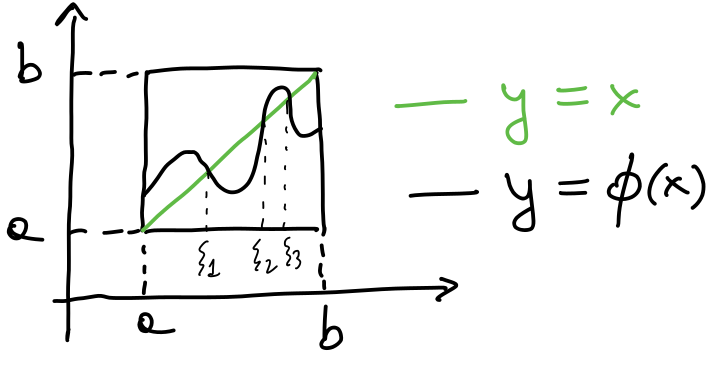
\includegraphics[width=0.5\textwidth]{img1_pag7.png}
\end{center}
ma se $\phi$ è una contrazione, l'unicità è assicurata. \\
Infatti se $\exists \xi_1, \xi_2 \in I$ con $\xi_1 \neq \xi_2$ tali che $\xi_1 = \phi(\xi_1)$ e $\xi_2 = \phi(\xi_2)$ allora $|\xi_1 - \xi_2| = |\phi(\xi_1) - \phi(\xi_2)| \leq \theta|\xi_1 - \xi_2|$ cioè $\theta \geq 1$ contro l'ipotesi che $\theta < 1$. \\
Resta da dimostrare che $\forall x_0 \in I$, definendo $x_{n+1} = \phi(x_n)$, $n \geq 0$ si ha $lim_{n\to\infty} \phi(x_n) = \xi$. \\
Ora $e_{n+1} = |x_{n+1} - \xi| = |\phi(x_n) - \phi(\xi)| \leq \theta|x_n - \xi| = \theta e_n$ da cui $e_1 \leq \theta e_0,$  $e_2 \leq \theta e_1 \leq \theta^2 e_0,$ $ \dotsc$,   $e_n \leq \theta^n e_0 \to 0, \ n\to\infty$ perché $\theta \in (0,1)$ \\
\vspace{0.5cm} \\
È il caso di fare subito alcune osservazioni importanti: \\
A) nel teorema delle contrazioni, la dimostrazione generale è basata sul fatto che la successione $\left\{ x_n \right\}$ è di Cauchy e quindi convergente a uno $\xi \in I$ (perché $I$ è chiuso) che è automaticamente punto fisso perché per continuità di $\phi$, $\xi = lim \ x_{n+1} = lim \ \phi(x_n) = \phi(lim \ x_n = \phi(\xi)$. \\
Ma anche con la dimostrazione scritta sopra, si ottiene la STIMA \underline{A PRIORI} dell'errore $e_n \leq \theta^n e_0$. \\
Se $\theta$ (ed $e_0$) sono noti questa permette a priori di stabilire il numero di iterazioni sufficiente ad ottenere $\xi$ con una tolleranza $\varepsilon > 0$, risolvendo la disuguaglianza
\begin{equation*}
    \theta^n e_0 \leq \varepsilon \Leftrightarrow e^{n\cdot log_{}{\theta}} \leq e^{log_{}{\frac{\varepsilon}{e_0}}} \Leftrightarrow n \geq \frac{log_{}{\frac{\varepsilon}{e_0}}}{log_{}{\theta}} = -\frac{log_{}{\frac{\varepsilon}{e_0}}}{|log_{}{\theta}|} = \frac{log_{}{\frac{e_0}{\varepsilon}}}{|log_{}{\theta}|}
\end{equation*}
visto che $\theta \in (0,1)$ e $log_{}{\theta} < 0$.\\
Notiamo che la convergenza e la stima ottenuta valgono $\forall x_0 \in I$, cioè le iterazioni di punto fisso che costruiscono (infinite) successioni diverse l'una dall'altra al variare di $x_0$, in ogni caso forniscono successioni che convergono tutte \underline{allo stesso limite} che è l'\underline{unico punto fisso} di $\phi$ in $I$, con una convergenza che è almeno lineare (ordine \underline{almeno} $p=1$) perché $e_{n+1} \leq \theta e_n$\\\\
B) si può facilmente ottenere una STIMA \underline{A POSTERIORI} dell'errore che spesso è più precisa della stima a priori: basta infatti scrivere: 
\begin{equation*}
    x_{n+1} - \xi = x_{n+1} - x_n + x_n - \xi
\end{equation*}
ma \[x_{n+1}-\xi -\phi(x_n) - \phi(\xi) \underset{\text{VALOR  MEDIO}}{\underset{\uparrow}{=}} \phi'(z_n)(x_n - \xi), \quad z_n \in int(x_n,\xi) \]
da cui \[ \phi'(z_n)(x_n - \xi) = x_{n+1}-x_n+x_n-\xi \]
ovvero \[ (1-\phi'(z_n))(x_n - \xi) = x_n-x_{n+1} \]
e passando ai moduli
\[\frac{|\,x_{n+1}-x_n\,|}{|\,1-\phi'(z_n)\,|} = e_n \le \frac{|\,x_{n+1}-x_n\,|}{1-\theta} \quad \Bigl( 1^\circ \text{ stima a posteriori}\Bigr)\]
perchè 
\begin{equation*}
    |\,\phi'(z_n)\,| \le \theta < 1 \Longrightarrow |\,1-\phi'(z_n)\,| \ge ||\,1-|\,\phi'(z_n)\,|| \ge 1 - \theta > 0
\end{equation*}
     e 
\begin{equation*}
    \frac{1}{|\,1-\phi'(z_n)\,|} \le \frac{1}{1-\theta}
\end{equation*}
In pratica abbiamo fatto vedere che l'errore è stimato dallo STEP $= |\,x_{n+1}-x_n\,|$ a meno del fattore $\frac{1}{(1-\theta)}=$ peso.\\
Se $\theta$ è piccolo, lo step diventa da solo una buona stima dell'errore perchè il peso è $\approx 1$; invece se $\theta$ è vicino ad 1, lo step va corretto per evitare una possibile sottostima.\\
Ma se $\phi \in C^1(I)$, siccome $z_n \to \xi$ allora $\phi'(z_n) \to \phi'(\xi)$, $n \to \infty$, quindi una stima a posteriori migliore è tendenzialmente la stima empirica (almeno per $n$ abbastanza grande)
\[e_n = \frac{|\,x_{n+1}-x_n\,|}{1-\phi'(z_n)} \approx \frac{|\,x_{n+1}-x_n\,|}{1-\phi'(x_n)} \quad \Bigl( 2^\circ \text{ stima a posteriori}\Bigr)\]
Conviene a questo punto fare un\\ \textbf{\underline{ESEMPIO}}\\
Consideriamo l'equazione in forma di punto fisso
\[x = \phi(x) = e^{-\alpha x}, \quad \alpha>0\]
se \underline{$\alpha<1$}, \[|\,\phi'(x)\,| = |\,-\alpha e^{-\alpha x}\,| \le \alpha < 1\]
e quindi $\phi$ contrae le distanze, cioè l'ipotesi (2) del teorema delle contrazioni è soddisfatta con $\phi = \alpha$; d'altra parte, $0<\phi(x) \le 1\, \forall x \in [0,+\infty)$, quindi anche (1) è soddisfatta con $I = [0,+\infty)$.\\
In realtà, siccome $\phi'(x)=-\alpha e^{-\alpha x}<0$, $\phi$ è strettamente decrescente (e positiva), quindi visto che $\phi(0)=1$ e $0<\phi(1)=1-e^{-\alpha}<1$ si ha
\[0 < \phi(x) \le 1 \quad \forall x \in [0,1]\]
cioè $\phi$ è anche una contrazione di $[a,b] = [0,1]$ in se stesso.\\
Allora $\exists$ un unico $\xi$ punto fisso di $\phi$ in $[0,1]$: prendiamo 
\[x_0 = \frac{1}{2} \Longrightarrow e_0 = |\,x_0 - \xi\,| \le \frac{1}{2}\]
e la successione $x_{n+1}=\phi(x_n)$, $n \ge 0$ converge a $\xi$ con la stima a priori dell'errore $e_n \le \frac{\alpha^n}{2}$.\\
Nel grafico qui sotto mostriamo l'errore effettivo, la stima a priori e la stima a posteriori dello step (non pesato) e dello step pesato da $\frac{1}{(1-\alpha)}$ e da $\frac{1}{(1-\phi'(x_n))}$ con
\[\alpha = 0.2 \Longrightarrow fl(\xi) = 0.8445798674955478\]
\[\alpha = 0.9 \Longrightarrow fl(\xi) = 0.5887032951482605\]
(questi valori sono stati calcolati con il metodo di Newton, si veda Lez.10-Es.2)
\begin{center}
    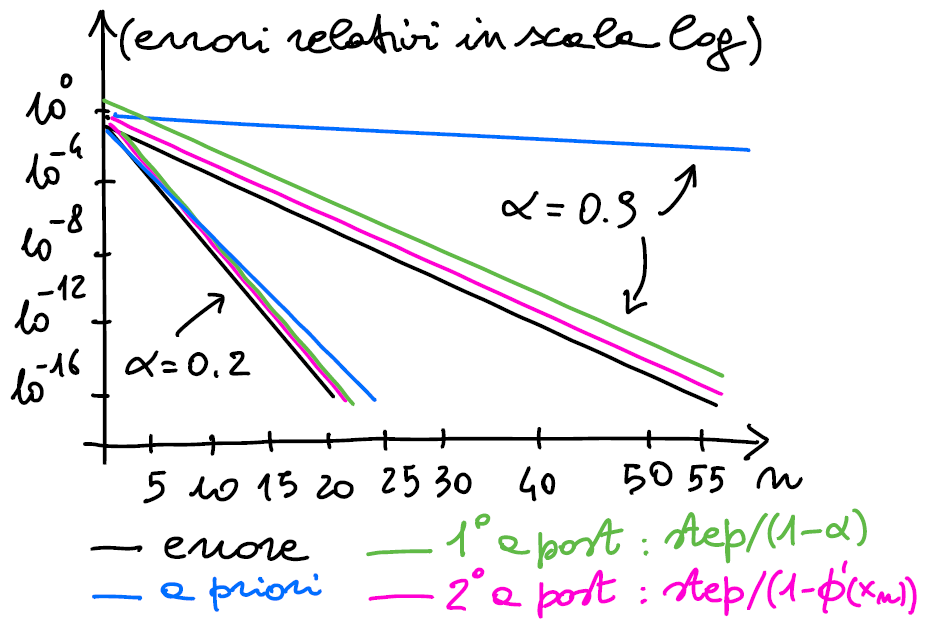
\includegraphics[width=0.8\textwidth]{pag16}
\end{center}
Si vede chiaramente che la convergenza è lineare, che la stima a priori è una sovrastima, molto distante dall'errore per $\alpha = 0.9$: infatti
\[\frac{e_{n+1}}{e_n} = |\,\phi'(z_n)\,| \to |\,\phi'(\xi)\,|, \quad n \to \infty \quad \text{cioè} \quad |\,\phi'(\xi)\,| = \alpha e^{-\alpha \xi} = L\]
è la costante asintotica, il parametro che effettivamente regola la velocità di convergenza ($\alpha$ è solo una stima) perchè per $n$ abbastanza grande
\[e_{n+1} \approx Le_n\]
Qui per $\alpha=0.9$ si ha $L \approx 0.53$ che è ben minore di $\alpha$, mentre per $\alpha=0.2$ si ha $L \approx 0.17$ che è poco minore di $\alpha$.\\
In effetti la $2^\circ$ stima a posteriori,
\[e_n = \frac{|\,x_{n+1} - x_n\,|}{(1 - \phi'(x_n))}\]
è una stima aderente dell'errore ma è shiftata in avanti di 1, fenomeno che abbiamo già visto nella stima con lo step nel metodo di Newton, perchè per stimare $e_n$ bisogna essere al passo $n+1$ (step = $|\,x_{n+1}-x_n\,|$)

\medskip
-------------- $\cdot$ --------------\\
Dopo aver discusso questo esempio semplice ma significativo, vediamo che anche per le iterazioni di punto fisso vale un risultato di \underline{convergenza locale} (mentre la formulazione generale del teorema delle contrazioni ha
carattere "globale", visto che $x_0 \in I$ è arbitrario e per la convergenza non è importante che $x_0$ sia vicino a $\xi$).

\bigskip
\textbf{TEOREMA (convergenza LOCALE delle iterazioni di punto fisso)}
\begin{center}
    \fbox{\begin{minipage}[t]{15cm} 
        Sia $\xi$ punto fisso di $\phi \in C^1(I_{\delta}(\xi))$ dove $I_{\delta}(\xi)=[\xi -\delta, \xi +\delta],\, \delta>0$ e sia $|\,\phi'(\xi)\,|<1$
        \begin{center}
                    $\Downarrow$ allora
        
        $\exists\, \delta'\le \delta : x_{n+1} = \phi(x_n), \, n\ge 0,$ converge a $\xi, \quad \forall\,x_0 \in I_{\delta'}(\xi)$
        \end{center}
    \end{minipage}}
\end{center}
È chiaro il carattere "locale" di questo risultato, che fornisce
condizioni sufficienti per la convergenza delle iterazioni di punto fisso purchè $x_0$ \underline{sia abbastanza vicino a $\xi$}.\\
\textbf{Dimostrazione (facoltativa)}\\
Siccome $\phi'$ è continua in $I_{\delta}(\xi)$ tale è $g(x)=|\phi'(x)|-1$, quindi visto che $g(\xi)<0$ per la permanenza del segno $\exists \, \delta'\le \delta$ tale che $g(x)<0$ $\forall x\in I_{\delta}'(\xi)$. Allora $\phi$ è una contrazione in $I_{\delta}'(\xi)$ con $\theta=\underset{x \in I_{\delta}'(\xi)}{max}|\phi'(x)|$, cioè vale l'ipotesi ($ii$) del teorema delle contrazioni con $I=I_{\delta'}(\xi)$; resta da far vedere che vale (1).\\
Ora, $\forall x \in I_{\delta'}(\xi)$
\begin{equation*}
    |\phi(x) - \xi| = |\phi(x) - \phi(\xi)| \leq \theta|x-\xi| \leq \theta \delta' < \delta'
\end{equation*}
cioè $\phi(x) \in I_\delta(\xi')\, \forall x \in I_{\delta'}(\xi)$ e quindi vale anche l'ipotesi (1) del teorema delle contrazioni. \\
Ne consegue che $\forall x_0 \in I_{\delta'}(\xi)$ la successione $x_{n+1} = \phi(x_n), \, n \ge 0$, converge a $\xi$, unico punto fisso di $\phi$ in $I_{\delta'}(\xi)$

\medskip
-------------- $\cdot$ --------------\\
Come per tutti i metodi iterativi, è importante capire quale sia l'\underline{ordine di convergenza} delle iterazioni di punto fisso.\\
Abbiamo già osservato che nel caso di una contrazione l'ordine è almeno $p=1$ perché vale\\ $e_{n+1}\leq\theta e_n \ con \ \theta \in (0,1)$.\\
D'altra parte, nell'esempio svolto prima, abbiamo fatto vedere che l'ordine è esattamente $p=1$ se $\phi'(\xi)\neq 0$ con costante asintotica $L=|\phi'(\xi)|$\\
Diamo ora una caratterizzazione completa col seguente:\\
\textbf{TEOREMA (ordine di convergenza delle iterazioni di punto fisso)}
\begin{center}
    \fbox{\begin{minipage}[t]{15cm}%
        Sia $\xi$ punto fisso di $\phi \in C^p(I),\ p \geq 1$ 
        con $I$ intervallo di $\mathbb{R}$ e supponiamo di essere in ipotesi che garantiscano la convergenza a $\xi$ di $x_{n+1}=\phi(x_n),\ n \geq 0,$ con\\ $x_0 \in I$ (ad esempio le ipotesi del teorema delle contrazioni) \\
        Allora:\\
        1) $\{x_n\}$ ha ordine esattamente $p=1 \ \iff 0<|\phi'(\xi)|<1$\\
        2) $\{x_n\}$ ha ordine esattamente $p>1 \ \iff \phi^{(j)}(\xi)=0, \ 1\leq j \leq p-1 \ e \ \phi^{(p)}(\xi)\neq 0$
    \end{minipage}}
\end{center}
\underline{Dimostrazione}\\
1) si dimostra subito visto che 
\[e_{n+1}=|\phi'(z_n)|e_n, \ z_n \in int(\xi,x_n)\]
per il teorema del valor medio, quindi 
\[\lim\limits_{n\to\infty} \frac{e_{n+1}}{e_n} = |\phi'(\lim z_n)|=|\phi'(\xi)|\]
per 2) utilizziamo la formula di Taylor di grado $p-1$ centrata in $\xi$ con resto p-esimo in forma di Lagrange \\
$x_{n+1}=\phi(x_n)=\underset{\xi}{\underset{\shortparallel}{\phi(\xi)}}+ \phi'(\xi)(x_n-\xi)+\frac{\phi''(\xi)}{2}(x_n-\xi)^2+...+\frac{\phi^{(p-1)}(\xi)}{(p-1)!}(x_n-\xi)^{p-1}+\frac{\phi^{(p)}(u_n)}{p!}(x_n-\xi)^p \ , \\ u_n \in int(\xi,x_n)$\\
\textbf{Dimostriamo prima $"\Leftarrow"$ (condizione sufficiente)}\\
se $\phi^{(j)}(\xi)=0, \ 1\leq j \leq p-1$ e $\phi^{(p)}(\xi)\neq 0$, da Taylor $x_{n+1}-\xi=\frac{\phi^{(p)}(u_n)}{p!}(x_n-\xi)^p$\\
e passando ai moduli
\[\frac{e_{n+1}}{e_n^p}=\frac{|\phi^{(p)}(u_n)|}{p!}\underset{n\to\infty}{\longrightarrow}\frac{|\phi^{(p)}(\xi)|}{p!}\neq 0\]
perché $u_n\rightarrow \xi$, $n\to\infty$ e $\phi^{(p)}$ è continua quindi $\lim \phi^{(p)}(u_n)=\phi^{(p)}(\lim u_n)=\phi^{(p)}(\xi)$\\
ovvero $\{x_n\}$ ha ordine esattamente $p$. \\
Per \textbf{dimostrare "$\Rightarrow$" (condizione necessaria)}\\ supponiamo per assurdo che $\lbrace x_n \rbrace $ abbia ordine esattamente $p$ ma che $\exists j<p$ tale che $\phi^{(j)}(\xi)\neq 0 $, prendiamo $k=min\lbrace j<p:\phi^{(j)}(\xi)\neq0\rbrace$ e scriviamo $\frac{e_{n+1}}{e_n^p} = \frac{e_{n+1}}{e_n^k}\cdot e_n^{k-p}$ \\
Ora per ipotesi $\frac{e_{n+1}}{e_n^p}\rightarrow L \neq 0$ ,\\
d'altra parte con lo stesso ragionamento usato per "$\Leftarrow$" tramite la formula di Taylor si avrebbe
\[\frac{e_{n+1}}{e_n^k}\rightarrow \frac{|\phi^{(k)}(\xi)|}{k!}=L'\neq 0\] 
ma allora
\[\frac{e_{n+1}}{e_n^p} = \frac{e_{n+1}}{e_n^k}\cdot e_n^{k-p}\]
\begin{center}
$\Bigl( \frac{e_{n+1}}{e_n^k} \to L' \text{ ed } e_n^{k-p} \to \infty \text{ perchè } k-p<0 \text{ ed } e_n \to 0 \Bigr)$    
\end{center}

cioè \[\frac{e_{n+1}}{e_n^p} \to \infty, \quad n \to \infty\]
contraddicendo l'ipotesi che abbia limite finito.

\medskip
-------------- $\cdot$ --------------\\
Ribadiamo che la condizione data è \underline{NECESSARIA} e \underline{SUFFICIENTE}, cioè fornisce una caratterizzazione completa di quando le iterazioni di punto fisso hanno ordine $p>0$.\\
In particolare (e questo ci servirà tra poco) le iterazioni di punto fisso possono avere convergenza \underline{quadratica} ($\phi'(\xi)=0$ e $\phi''(\xi)\ne 0$), \underline{cubica} ($\phi'(\xi)=\phi''(\xi)=0$ e $\phi'''(\xi)\ne0, \dotsc$).

\bigskip
Per concludere la lezione, mostriamo infatti che il metodo di Newton si può re-interpretare come iterazione di punto fisso e che, in base a quanto visto sopra, si vede subito che ammette convergenza locale e che la convergenza è quadratica per zeri semplici.\\
Infatti l'iterazione di Newton
\[x_{n+1} = x_n - \frac{f(x_n)}{f'(x_n)}, \quad n\ge 0\]
è di tipo punto fisso con
\[\phi(x) = x - \frac{f(x)}{f'(x)}\]
e se $f \in C^k(I)$ con $f'(x)\ne 0 \,\forall x \in I$ intervallo, allora $\phi \in C^{k-1}(I)$.\\
È evidente che $\xi$ è zero (semplice) di $f \iff \xi$ è punto fisso di $\phi$.\\
Inoltre, il teorema di convergenza \underline{locale} per \underline{Newton} (zeri semplici) discende immediatamente dal teorema di convergenza \underline{locale} per le \underline{iterazioni di punto fisso} se $f \in C^2(I_\delta(\xi))$, infatti
\[ \phi'(x) = \frac{d}{dx}\biggl(x-\frac{f}{f'}\biggr) = 1 - \underbrace{\frac{(f')^2 - ff''}{(f')^2}}_{\text{derivata\, del\,rapporto}} = \frac{ff''}{(f')^2}\]
quindi $f(\xi)=0 \Rightarrow \phi'(\xi)=0$ e $|\phi'(\xi)|=0<1$, allora $\exists\, \delta'\le \delta$ tale che l'iterazione di Newton converge come iterazione di punto fisso $\forall x_0 \in I_{\delta'}(\xi)$.\\
D'altra parte, sempre interpretando Newton come iterazione di punto fisso, è immediato che la convergenza per zeri semplici è almeno quadratica perché $\phi'(\xi)=0$ ed è esattamente quadratica se $f''(\xi)\neq0$, utilizzando la caratterizzazione vista sopra (che però richiede $\phi \in C^2$ e quindi $f\in C^3$) infatti:
\begin{equation*}
    \phi''=\frac{d}{dx}\biggl(\frac{f f''}{(f')^2}\biggr)= 
    \underbrace{\frac{\overset{ \downarrow \ derivata \ del \ prodotto}{(f' f''+f f''')(f')^2-2 f' f'' (f f'')}}{(f')^4}}_{\text{ancora\, derivata\, del\, rapporto}}
\end{equation*}
da cui 
\begin{equation*}
    \phi''(\xi)=\frac{f''(\xi)}{(f'(\xi))^3}\neq 0
\end{equation*}
perché 
\begin{equation*}
    f''(\xi)\neq 0 \ ( e \ f'(\xi)\neq0)
\end{equation*}
Non è difficile vedere (come approfondimento facoltativo) che interpretando Newton come iterazione di punto fisso, nel caso di zero multiplo l'ordine di convergenza diventa $p=1$ con costante asintotica $|\phi'(\xi)|=1-\frac{1}{m}$ dove $m$ è la molteplicità di $\xi$ (il numero di derivate successive che si annullano in $\xi$) e che se $m$ è nota, l'iterazione
\[x_{n+1}=x_n-m\frac{f(x_n)}{f'(x_n)}=\phi_m(x_n)\]
torna di ordine almeno $p=2$ perché 
\[\phi'_m(\xi)=\lim\limits_{x\to\xi}\phi'_m(x)=0\]

\end{document}

